% Related Work

\chapter{Related Work and Used Technologies} % Main chapter title

\label{chapter2_bg}
This chapter presents some background for the content of this thesis.

\section{Related Work}

\subsection{Plotly}
Plotly is a popular public data visualizationcloud service provider. Plotly provides community, professional and enterprise data storage, visualization and analytics services to the user.  Excel, CSV and XML data formats are used to upload the data to its cloud servers.  Plotly provides online graphing, analytics, and statistics tools for individuals and collaboration, as well as scientific graphing libraries for Python, R, MATLAB, Perl, Julia, Arduino, and REST.

\subsection{Loopback}
LoopBack is a highly-extensible, open-source Node.js framework which assimilates the best practices of model driven software develpment. LoopBack simplifies and speeds up REST API development. It consists of a library of Node.js modules for connecting web and mobile apps to data sources such as databases and REST APIs, a command line tool, and client-SDKs. A loopback application has three components: models that represent business data and behavior, data sources and connectors, and mobile clients.An application interacts with data sources through the LoopBack model API, available locally within Node, remotely over REST, and via native client APIs for iOS, Android, and HTML5. Using the API, apps can query databases, store data, upload files, send emails, create push notifications, register users, and perform other actions provided by data sources.
	Loopback is implemented with many of the technologies we use in this thesis. It uses MDSD as a general practice, data access objects for the communication between database and the REST API, access control list for  authorization and is written in Node.js.

\section{Used Technologies}

\subsection{HTML5}
HTML5~\cite{pilgrim2010html5} is a markup language used for structuring and presenting content on the World Wide Web. It is the fifth and current major version of the HTML standard.\par
It was published in October 2014 by the World Wide Web Consortium (W3C) to improve the language with support for the latest multimedia, while keeping it both easily readable by humans and consistently understood by computers and devices such as web browsers, parsers, etc. HTML5 is intended to subsume not only HTML 4, but also XHTML 1 and DOM Level 2 HTML.\par
HTML5 includes detailed processing models to encourage more interoperable implementations; it extends, improves and rationalizes the markup available for documents, and introduces markup and application programming interfaces (APIs) for complex web applications. For the same reasons, HTML5 is also a candidate for cross-platform mobile applications, because it includes features designed with low-powered devices in mind.

\subsection{CSS3}
Cascading Style Sheets (CSS) is a style sheet language used for describing the presentation of a document written in a markup language. Although most often used to set the visual style of web pages and user interfaces written in HTML and XHTML, the language can be applied to any XML document, including plain XML, SVG and XUL, and is applicable to rendering in speech, or on other media. Along with HTML and JavaScript, CSS is a cornerstone technology used by most websites to create visually engaging webpages, user interfaces for web applications, and user interfaces for many mobile applications.\par
CSS is designed primarily to enable the separation of presentation and content, including aspects such as the layout, colors, and fonts. This separation can improve content accessibility, provide more flexibility and control in the specification of presentation characteristics, enable multiple HTML pages to share formatting by specifying the relevant CSS in a separate .css file, and reduce complexity and repetition in the structural content. CSS3~\cite{mcfarland2012css3} is the latest version of CSS and used in this thesis.


\subsection{Javascript}
JavaScript (JS)~\cite{crockford2008javascript}, is a high-level, dynamic, weakly typed, object-based, multi-paradigm, and interpreted programming language. Alongside HTML and CSS, JavaScript is one of the three core technologies of World Wide Web content production. It is used to make webpages interactive and provide online programs, including video games. As a multi-paradigm language, JavaScript supports event-driven, functional, and imperative (including object-oriented and prototype-based) programming styles. Initially only implemented client-side in web browsers, JavaScript engines are now embedded in many other types of host software, including server-side in web servers and databases. The most famous server-side Javascript implementation is Node.js.

\subsubsection{Node.js}
\begin{figure}
	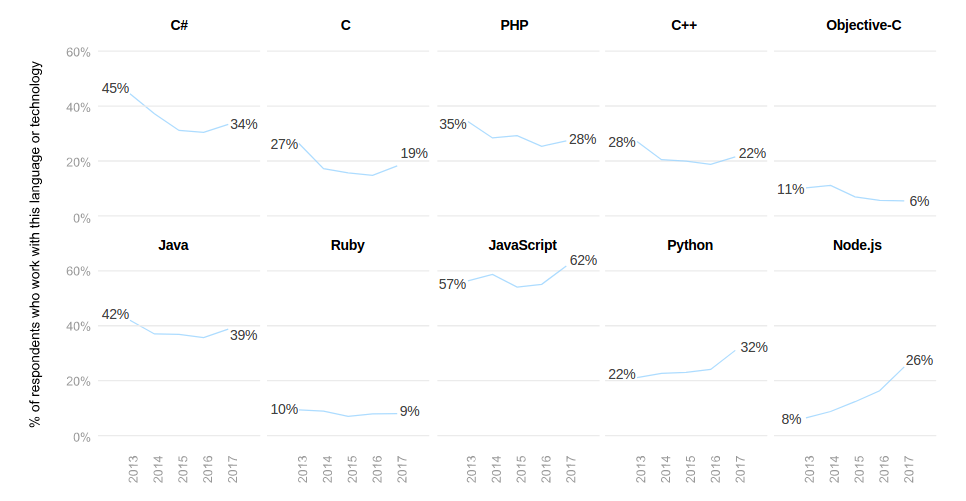
\includegraphics[scale=0.5]{survey17.png}
	\caption{Developers survey for Stack Overflow website in 2017.}
	\label{survey17}
\end{figure}
Node.js~\cite{tilkov2010node} is an open-source, cross-platform JavaScript run-time environment for executing JavaScript code server-side.Node.js provides an event-driven architecture and a non-blocking I/O API designed to optimize application's throughput and scalability for real-time Web applications. It uses Google V8 JavaScript engine to execute code, and a large percentage of the basic modules are written in JavaScript. Node.js contains a built-in library to allow applications to act as a stand-alone Web server. The increasing popularity of Node.js in the last years can be seen in figure~\ref{survey17}.

\subsubsection{JSON}
\label{json}
In computing, JavaScript Object Notation or JSON~\cite{crockford2006application}, is an open-standard file format that uses human-readable text to transmit data objects consisting of attribute–value pairs and array data types (or any other serializable value). It is a very common data format used for asynchronous browser/server communication, including as a replacement for XML in some AJAX-style systems.
JSON is a language-independent data format. It was derived from JavaScript, but as of 2017 many programming languages include code to generate and parse JSON-format data. The official Internet media type for JSON is application/json. JSON filenames use the extension .json. JSON's basic data types are described below. \par
\paragraph{Number} A signed decimal number that may contain a fractional part and may use exponential E notation, but cannot include non-numbers like NaN. The format makes no distinction between integer and floating-point. JavaScript uses a double-precision floating-point format for all its numeric values, but other languages implementing JSON may encode numbers differently.
\paragraph{String} A sequence of zero or more Unicode characters. Strings are delimited with double-quotation marks and support a backslash escaping syntax.
\paragraph{Boolean} Either of the values true or false.
\paragraph{Array} An ordered list of zero or more values, each of which may be of any type. Arrays use square bracket notation with elements being comma-separated.
\paragraph{Object} An unordered collection of name/value pairs where the names (also called keys) are strings. Since objects are intended to represent associative arrays, it is recommended, though not required, that each key is unique within an object. Objects are delimited with curly brackets and use commas to separate each pair, while within each pair the colon ':' character separates the key or name from its value.
\paragraph{null} An empty value, using the word null.

\subsubsection{Ajax}
\label{ajax}
\begin{figure}
	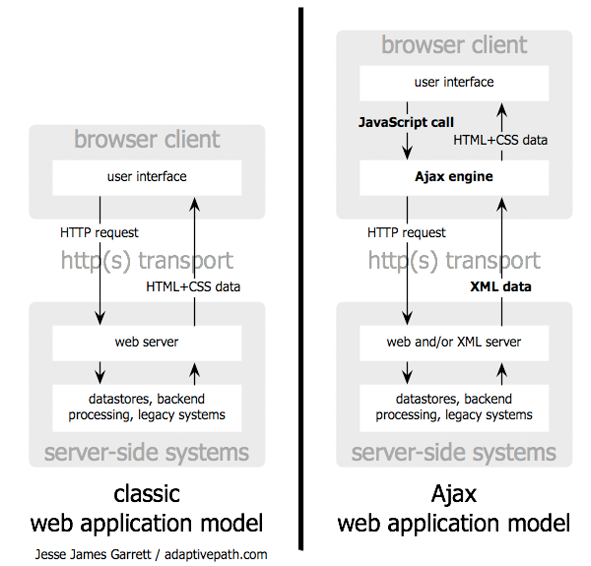
\includegraphics[scale=0.7]{ajax.png}
	\caption{The traditional model for web applications (left) compared to the Ajax model (right)}
	\label{ajaxPNG}
\end{figure}
Ajax (short for "asynchronous JavaScript and XML")~\cite{garrett2005ajax} is a set of Web development techniques using many Web technologies on the client side to create asynchronous Web applications. With Ajax, Web applications can send data to and retrieve from a server asynchronously (in the background) without interfering with the display and behavior of the existing page. By decoupling the data interchange layer from the presentation layer, Ajax allows for Web pages, and by extension Web applications, to change content dynamically without the need to reload the entire page. In practice, modern implementations commonly substitute JSON for XML due to the advantages of being native to JavaScript.\par
Ajax is not a single technology, but rather a group of technologies. HTML and CSS can be used in combination to mark up and style information. The DOM is accessed with JavaScript to dynamically display – and allow the user to interact with – the information presented. JavaScript and the XMLHttpRequest object provide a method for exchanging data asynchronously between browser and server to avoid full page reloads.\par 
The term Ajax has come to represent a broad group of Web technologies that can be used to implement a Web application that communicates with a server in the background, without interfering with the current state of the page, such as HTML, CSS, DOM, XMLHttpRequest etc. The conventional model for a Web Application versus an application using Ajax can be seen in figure~\ref{ajaxPNG}.

\subsubsection{Node Package Manager}
Npm~\cite{schlueternode} is a package manager for the JavaScript programming language. It is the default package manager for the JavaScript runtime environment Node.js. It consists of a command line client, also called npm, and an online database of public packages, called the npm registry. The registry is accessed via the client, and the available packages can be browsed and searched via the npm website. Npm is included as a recommended feature in Node.js installer. Npm consists of a command line client that interacts with a remote registry. It allows users to consume and distribute JavaScript modules that are available on the registry. Packages on the registry are in CommonJS format and include a metadata file in JSON format.

\subsection{NoSQL Database}
A NoSQL (originally referring to "non SQL" or "non relational")[1] database provides a mechanism for storage and retrieval of data that is modeled in means other than the tabular relations used in relational databases.NoSQL databases are increasingly used in big data and real-time web applications.Motivations for this approach include: simplicity of design, simpler "horizontal" scaling to clusters of machines (which is a problem for relational databases), and finer control over availability. The data structures used by NoSQL databases (e.g. key-value, wide column, graph, or document) are different from those used by default in relational databases, making some operations faster in NoSQL. The particular suitability of a given NoSQL database depends on the problem it must solve. Sometimes the data structures used by NoSQL databases are also viewed as "more flexible" than relational database tables.

\subsubsection{MongoDB}
MongoDB is a free and open-source cross-platform document-oriented database program. Classified as a NoSQL database program, MongoDB uses JSON-like documents with schemas.


